\setcounter{page}{2}


\textbf{Тик} -- период времени между двумя последующими прерываниями таймера.

\textbf{Основной тик} -- период времени равный n тикам таймера (число n
зависит от конкретного варианта системы).

\textbf{Квант времени} (quantum, time slice) — временной интервал, в течение которого процесс может использовать процессор до вытеснения другим процессом.

\chapter{Функции обработчика прерывания от системного таймера в защищенном режиме}

Обработчик прерываний от системного таймера имеет наивысший приоритет. Никакая другая работа в системе не может выполняться во время обработчика прерывания от системного таймера. Обработчик прерывания от системного таймера должен завершаться как можно быстрее, чтобы не влиять на отзывчивость системы (отзывчивость – как быстро система отвечает на запросы пользователей).

\section{Unix} %\cite{unix}
\subsection*{По тику}

\begin{itemize}
	\item инкремент счетчика тиков аппаратного таймера
	\item инкремент счетчика использование процессора текущим процессом (то есть инкремент поля p\_cpu структуры proc до максимального значения -- 127)
	\item инкремент часов и других таймеров системы
	\item декремент кванта текущего потока
	\item декремент счетчика времени до отправления на выполнение отложенных вызовов, при достижении счетчиком нуля происходит выставление флага для обработчика отложенного вызова [1]%\cite{unix}
\end{itemize}

\subsection*{По главному тику}

\begin{itemize}
	\item пробуждает в нужные моменты системные процессы, такие как swapper и pagedaemon. ('пробуждает' тут понимается так: инициирование отложенного вызова процедуры wakeup, которая перемещает дескрипторы процессов из списка "спящие" в очередь готовых к выполнению)
	\item инициирует отложенные вызовы функции, которые относятся к работе планировщика
	
	
	\item декрементирует счетчик времени, которое осталось до отправления одного из следующих сигналов:
	\begin{itemize}
		\item SIGVTALRM – сигнал, посылаемый процессу по истечении времени, заданного в “виртуальном” таймере;
		\item SIGPROF – сигнал, посылаемый процессу по истечении времени заданного в таймере профилирования;
		\item SIGALRM – сигнал, посылаемый процессу по истечении времени, предварительно заданного функцией alarm().	
	\end{itemize}
\end{itemize}

\subsection*{По кванту}

\begin{itemize}
	\item посылка текущему процессу сигнала SIGXCPU, если он превысил выделенную для него квоту использования процессора. По получению сигнала обработчик сигнала прерывает выполнение процесса.
\end{itemize}


\section{Windows}

\subsection*{По тику}
\begin{itemize}
	\item инкремент счетчика системного времени
	\item декремент счетчиков времени отложенных задач
	\item декремент кванта текущего потока %(декремент происходит на величину, равную кол-ву тактов процессора, произошедших за тик. В случае, если количество затраченных потомков тактов процессора достигает квантовой цели, запускается обработка истечения кванта)
	\item Если активен механизм профилирования ядра, то инициализация отложенного вызова обработчика ловушки профилирования ядра с помощью постановки объекта в очередь DPC (обработчик ловушки профилирования регистрирует адрес команды, выполнявшейся на момент прерывания)
\end{itemize}

\subsection*{По главному тику}
\begin{itemize}
	\item Освобождение объекта «событие», которое ожидает диспетчер настройки баланса. (Диспетчер настройки баланса по событию от таймера сканирует очередь готовых процессов и повышает приоритет процессов, которые находились в состоянии ожидания дольше 4 секунд.)
\end{itemize}

\subsection*{По кванту}
\begin{itemize}
	\item Инициация диспетчеризации потоков (добавление соответствующего объекта в очередь DPC -- Deferred procedure call — отложенный вызов процедуры)
\end{itemize}

\chapter{Пересчет динамических приоритетов}

В ОС семейства UNIX и в ОС семейства Windows только \textbf{приоритеты пользовательских процессов} могут динамически пересчитываться.
\section{Unix}

Планирование процессов в UNIX основано на приоритете процесса. Планировщик всегда выбирает процесс с наивысшим приоритетом. Приоритеты процессоров изменяются динамически системой в зависимости от использования вычислительных ресурсов, времени ожидания запуска и текущего состояния процесса. Если процесс готов к запуску и имеет наивысший приоритет, планировщик приостановит выполнение текущего процесса (с более низким приоритетом), даже если тот не «выработал» свой временной квант.

Традиционное ядро UNIX является строго невытесняющим, однако в современных системах UNIX ядро является вытесняющим -- то есть процесс в режиме ядра может быть вытеснен более приоритетным процессом в режиме ядра. Ядро сделано вытесняющим для того, чтобы система могла обслуживать процессы реального времени, например видео и аудио.

Очередь процессов, готовых к выполнению, формируется согласно приоритетам и принципу вытесняющего циклического планирования, то есть сначала выполняются процессы с большим приоритетом, а процессы с одинаковым приоритетом выполняются в течении кванта времени друг за другом циклически. В случае, если процесс с более высоким приоритетом поступает в очередь процессов, готовых к выполнению, планировщик вытесняет текущий процесс и предоставляет ресурс более приоритетному процессу.

Приоритет процесса задается любым целым числом, которое лежит в диапазоне от 0 до 127 (чем меньше число, тем выше приоритет)
\begin{itemize}
	\item 0 - 49 -- зарезервированы для ядра (приоритеты ядра фиксированы)
	\item 50 - 127 -- прикладные  (приоритеты прикладных задач могут изменяться во времени)
\end{itemize}

Изменение приоритета прикладных задач зависит от следующих факторов:
\begin{itemize}
	\item \textbf{фактор ”любезности” (nice)} -- это целое число в диапазоне от 0 до 39 со значением 20 по умолчанию. Увеличение значения приводит к уменьшению приоритета. Пользователи могут повлиять на приоритет процесса при помощи изменения значений этого фактора, но только суперпользователь может увеличить приоритет процесса. Фоновые процессы автоматически имеют более высокие значения этого фактора.
	\item \textbf{последней измеренной величины использования процессора} 
\end{itemize}


Структура proc содержит следующие поля, которые относятся к приоритетам:
\begin{itemize}
	\item p\_pri -- текущий приоритет планирования
	\item p\_usrpri -- приоритет режима задачи
	\item p\_cpu -- результат последнего измерения использования процессора
	\item p\_nice -- фактор 'любезности', который устанавливается пользователем
\end{itemize}

\textbf{p\_pri} используется планировщиком для принятия решения о том, какой процесс отправить на выполнение. \textbf{p\_pri} и \textbf{p\_usrpri} равны, когда процесс находится в режиме задачи. 

Значение \textbf{p\_pri} может быть изменено (повышено) планировщиком для того, чтобы выполнить процесс в режиме ядра. В таком случае \textbf{p\_usrpri} будет использоваться для хранения приоритета, который будет назначен процессу при возврате в режим задачи.

\textbf{p\_cpu} инициализируется нулем при создании процесса (и на каждом тике обработчик таймера увеличивает это поле текущего процесса на 1, до максимального значения равного 127).

Ядро системы связывает приоритет сна с событием или ожидаемым ресурсом, из-за которого процесс может блокироваться (приоритет сна определяется для ярда, поэтому лежит в диапазоне 0 - 49). Когда процесс ”просыпается”, ядро устанавливает в поле \textbf{p\_pri} приоритет сна – значение приоритета из диапазона системных приоритетов, зависящее от события или ресурса по которому произошла блокировка. (событие и связанное с ним значение приоритета сна в системе 4.3BSD представлены в таблице \ref{tab:bsd}).


\begin{table}[h]
	\caption{Приоритеты
		сна в ОС \textbf{4.3BSD} (из книги [1] ”UNIX изнутри”)}
	\label{tab:bsd}
	\begin{center}
		\begin{tabular}{ |c|c|c|  }
			\hline
			\textbf{Приоритет} & \textbf{Значение} & \textbf{Описание} \\
			\hline
			\texttt{PSWP} & 0 & Свопинг \\
			\hline
			\texttt{PSWP + 1} & 1 & Страничный демон \\
			\hline
			\texttt{PSWP + 1/2/4} & 1/2/4 & Другие действия по обработке памяти \\
			\hline
			\texttt{PINOD} & 10 & Ожидание освобождения inode \\
			\hline
			\texttt{PRIBIO} & 20 & Ожидание дискового ввода-вывода \\
			\hline
			\texttt{PRIBIO + 1} & 21 & Ожидание освобождения буфера \\
			\hline
			\texttt{PZERO} & 25 & базовый приоритет \\
			\hline
			\texttt{TTIPRI} & 28 & Ожидание ввода с терминала \\
			\hline
			\texttt{TTOPRI} & 29 & Ожидание вывода с терминала \\
			\hline 
			\texttt{PWAIT} & 30 & Ожидание завершения процесса потомка \\
			\hline
			\texttt{PLOCK} & 35 & Консультативное ожидание блок. ресурса \\
			\hline
			\texttt{PSLEP} & 40 & Ожидание сигнала \\
			\hline
		\end{tabular}
	\end{center}
\end{table}

Также приведена таблица из книги ”Операционная система UNIX” Андрея Робачевского на рисунке 2.1. Заметим, что направление роста значений приоритета для этих систем (4.3BSD UNIX и SCO UNIX) различно.

\captionsetup{justification=centering, singlelinecheck=false}
\begin{figure}[H]
	\centering
	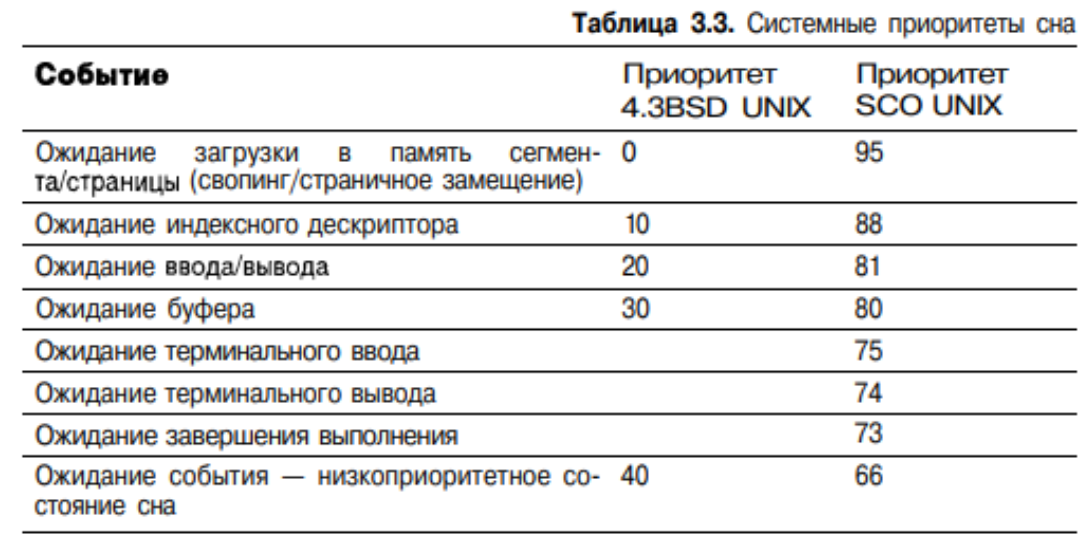
\includegraphics[width=1\linewidth]{inc/img/priors}
	\caption{Системные приоритеты сна}
	\label{fig:demographics1}
\end{figure}

Каждую секунду ядро системы инициализирует отложенный вызов процедуры schedcpu(), которая уменьшает значение \textbf{p\_pri} каждого процесса исходя из фактора ''полураспада'' (в системе 4.3BSD считается по формуле \ref{eq:ref1})

\begin{equation}
\label{eq:ref1}
decay = \frac{2 \cdot load\_average}{2 \cdot load\_average + 1}
\end{equation} где
\textit{load\_average} -- это среднее количество процессов, находящихся в состоянии готовности к выполнению, за последнюю секунду.

Также процедура schedcpu() пересчитывает приоритеты для режима задачи
всех процессов по формуле \ref{eq:ref2},

\begin{equation}
\label{eq:ref2}
p\_usrpri = PUSER + \frac{p\_cpu}{2} + 2 \cdot p\_nice
\end{equation}где \textit{PUSER} - базовый приоритет в режиме задачи, равный 50.

Таким образом, если процесс в последний раз использовал большое количество процессорного времени, то его \textbf{р\_срu} будет увеличен. Это приведет к росту значения \textbf{p\_usrpri}, то есть к понижению приоритета. Чем дольше процесс простаивает в очереди на выполнение, тем больше фактор полураспада уменьшает его \textbf{р\_срu}, что приводит к повышению его приоритета. Такая схема предотвращает бесконечное откладывание низкоприоритетных процессов. Применение данной схемы предпочтительно процессам, осуществляющим много операций ввода-вывода, в противоположность процессам, производящим много вычислений.

То есть, если процесс большинство времени выполнения тратит на ожидание ввода-вывода, то он остается с высоким приоритетом и, таким образом, быстрее получает процессор при необходимости.

В тоже время вычислительные приложения обычно обладают более высокими значениями \textbf{р\_срu} и работают на значительно более низких приоритетах.


\textbf{Динамический пересчет приоритетов процессов в режиме задачи позволяет избежать бесконечного откладывания.}

Таким образом, приоритет процесса в режиме задачи может быть динамически пересчитан по следующим причинам:

\clearpage

\begin{itemize}
	\item Вследствие изменения фактора любезности процесса системным вызовом nice
	\item В зависимости от степени загруженности процессора процессом p\_cpu
	\item Вследствие ожидания процесса в очереди готовых к выполнению процессов
	\item Приоритет может быть повышен до соответствующего приоритета сна вследствие ожидания ресурса или события
\end{itemize}


\section{Windows}

В Windows процессу при создании назначается базовый приоритет. Относительно
базового приоритета процесса потоку назначается относительный приоритет.

Планирование осуществляется только на основании приоритетов потоков, готовых
к выполнению: если поток с более высоким приоритетом становится готовым к выполнению, поток с более низким приоритетом вытесняется планировщиком. По истечению кванта времени текущего потока, ресурс передается самому приоритетному потоку в
очереди готовых к выполнению

Windows использует 32 уровня приоритета:
\begin{itemize}
	\item от 0 до 15 -- 16 изменяющихся уровней (из которых уровень 0 -- зарезервирован для потока обнуления страниц)
	\item от 16 до 31 -- 16 уровней реального времени
\end{itemize}

Уровни приоритета потоков назначаются исходя из двух разных позиций: одной от Windows API и другой от ядра Windows. Сначала Windows API систематизирует процессы по классу приоритета, который им присваивается при создании:
\begin{itemize}
	\item Реального времени — Real-time (4)
	\item Высокий — High (3)
	\item Выше обычного — Above Normal (6)
	\item Обычный — Normal (2)
	\item Ниже обычного — Below Normal (5)
	\item Простоя — Idle (1)
\end{itemize}

После назначается относительный приоритет отдельных потоков внутри этих процессов
\begin{itemize}
	\item Критичный по времени — Time-critical (15)
	\item Наивысший — Highest (2)
	\item Выше обычного — Above-normal (1)
	\item Обычный — Normal (0)
	\item Ниже обычного — Below-normal (–1)
	\item Самый низший — Lowest (–2)
	\item Простоя — Idle (–15)
\end{itemize}

Исходный базовый приоритет потока наследуется от базового приоритета процесса. Процесс по умолчанию наследует свой базовый приоритет у того процесса, который его создал. Соответствие между приоритетами Windows API и ядра системы приведено в таблице \ref{tbl:priority}


\begin{table}[h]
	\caption{Соответствие между приоритетами \textbf{Windows API} и ядра Windows}
	\begin{center}
		\begin{tabular}{|l|p{45pt}|p{45pt}|p{45pt}|p{45pt}|p{45pt}|p{45pt}|}
			\hline
			{} & \textbf{real-time} & \textbf{high} & \textbf{above normal} & \textbf{normal} & \textbf{below normal} & \textbf{idle}\\
			\hline
			\textbf{time critical} & 31 & 15 & 15 & 15 & 15 & 15 \\
			\hline
			\textbf{highest} & 26 & 15 & 12 & 10 & 8 & 6 \\
			\hline
			\textbf{above normal} & 25 & 14 & 11 & 9 & 7 & 5 \\
			\hline
			\textbf{normal} & 24 & 13 & 10 & 8 & 6 & 4 \\
			\hline
			\textbf{below normal} & 23 & 12 & 9 & 7 & 5 & 3 \\
			\hline
			\textbf{lowest} & 22 & 11 & 8 & 6 & 4 & 2 \\
			\hline
			\textbf{idle} & 16 & 1 & 1 & 1 & 1 & 1 \\
			\hline
		\end{tabular}
	\end{center}
	\label{tbl:priority}
\end{table}

Текущий приоритет потока в динамическом диапазоне – от 1 до 15 – может быть повышен планировщиком вследствие следующих причин:

\begin{itemize}
	\item повышение вследствие событий планировщика или диспетчера (сокращение задержек);
	
	\item повышения приоритета, связанные с завершением ожидания;
	
	\item повышение приоритета владельца блокировки;
	
	\item Повышение вследствие завершения ввода-вывод;

	\begin{table}[h!]
		\caption{Рекомендуемые значения повышения приоритета.}
		\begin{center}
			\begin{tabular}{|p{100mm}|l|}
				\hline
				\textbf{Устройство} & \textbf{Приращение} \\
				\hline
				Диск, CD-ROM, параллельный порт, видео & 1 \\
				\hline
				Сеть, почтовый ящик, именованный канал, последовательный порт & 2 \\
				\hline
				Клавиатура, мышь & 6 \\
				\hline
				Звуковая плата & 8 \\
				\hline
			\end{tabular}
		\end{center}
		\label{tab:io}
	\end{table}
	
	\item повышение при ожидании ресурсов исполняющей системы;
	
	\item повышение приоритета потоков первого плана после ожидания;

	\item повышение приоритета после пробуждения GUI-потока;
	
	\item повышения приоритета, связанные с перезагруженностью центрального процессора;

	\item повышение приоритетов для мультимедийных приложений и игр;
	
		Потоки, на которых выполняются различные мультимедийные приложения, должны выполняться с минимальными задержками. В Windows такая задача решается с помощью повышения приоритетов таких потоков драйвером \textbf{MMCSS (MultiMedia Class Scheduler Service)}. MMCSS работает с различными определенным задачи, например:
		\begin{itemize}
			\item аудио
			\item аудио профессионального качества
			\item игры
			\item захват
			\item воспроизведение
			\item низкая задержка
			\item задачи администратора многооконного режима.
			\item распределение
		\end{itemize}
\end{itemize}



Важное свойство для планирования потоков -- категория планирования -- это первичный фактор, который определяет приоритет потоков, зарегистрированных с MMCSS (категории планирования указаны в таблице \ref{tab:plan}).

Функции MMCSS временно повышают приоритет потоков, зарегистрированных с MMCSS до уровня, который соответствует категории планирования. Потом их приоритет снижается до уровня, соответствующего категории планирования Exhausted, для того, чтобы другие потоки тоже могли получить ресурс.


\begin{table}[h]
	\caption{Категории планирования.}
	\begin{center}
		\begin{tabular}{|p{30mm}|p{30mm}|p{90mm}|}
			\hline
			\textbf{Категория} & \textbf{Приоритет} & \textbf{Описание} \\
			\hline
			High (Высокая) & 23-26 & Потоки профессионального аудио (Pro Audio), запущенные с приоритетом выше, чем у других потоков на системе, за исключением критических системных потоков \\
			\hline
			Medium (Средняя) & 16-22 & Потоки, являющиеся частью приложений первого плана, например Windows Media Player \\
			\hline
			Low (Низкая) & 8-15 & Все остальные потоки, не являющиеся частью предыдущих категорий \\
			\hline
			Exhausted (Исчерпавших потоков) & 1-7 & Потоки, исчерпавшие свою долю времени центрального процессора, выполнение которых продолжится, только если не будут готовы к выполнению другие потоки с более высоким уровнем приоритета \\
			\hline
		\end{tabular}
	\end{center}
	\label{tab:plan}
\end{table}

\chapter{Вывод}
Функции обработчика прерывания от системного таймера в защищенном режиме для ОС семейства UNIX и для OC семейства Windows схожи, так как эти ОС являются системами разделения времени. Общие основные функции:
\begin{itemize}
	\item декремент кванта текущего процесса в UNIX и декремент текущего потока в Windows.
	\item инициализация отложенных действий, которые относятся к работе планировщика (например пересчет приоритетов).
	\item декремент счетчиков времени (таймеров, часов, счетчиков времени отложенных действий, будильников реального времени ) 
\end{itemize}

Обе операционные системы (UNIX и Windows) -- это системы разделения времени с вытеснением и динамическими приоритетами.

В ОС UNIX приоритет пользовательского процесса (процесса в режиме задач) может динамически пересчитываться, в зависимости от фактора ''любезности'', p\_cpu (результат последнего измерения использования процессора) и базового приоритета (PUSER). Приоритеты ядра -- фиксированные величины.

В ОС Windows при создании процесса ему назначается базовый приоритет, относительно базового приоритета процесса потоку назначается относительный приоритет, таким образом, у потока нет своего приоритета. Приоритет потока пользовательского процесса может быть динамически пересчитан.








